\documentclass[11pt,a4paper]{article}

\usepackage[left=2cm,text={17cm,24cm},top=3cm]{geometry}
\usepackage[bookmarksopen,colorlinks,plainpages=false,urlcolor=blue,unicode,linkcolor=blue]{hyperref}
\usepackage[slovak]{babel}
\usepackage[utf8]{inputenc}
\usepackage[T1]{fontenc}
\usepackage{indentfirst}
\usepackage{graphicx}
\usepackage{enumitem}
\usepackage{float}
\usepackage{url}

\graphicspath{{.}}

\begin{document}

% #################################################################################################
% TITLEPAGE

\begin{titlepage}
    \begin{center}
        \Huge
        \textsc{
            Fakulta informačních technologií\\
            Vysoké učení technické v~Brně
        }
        \vspace{100px}
        \begin{figure}[!h]
            \centering
            
\includegraphics[scale=0.3]{img/vutbr-fit-logo.eps}
        \end{figure}
        \\[20mm]
        \huge{
            \textbf{
                IMP - Mikroprocesorové a vstavané systémy
            }
        }
        \\[2em]
        \LARGE{
            \textbf{
                Hodiny s budíkem na bázi modulu\\
                Real Time Clock (RTC)
            }
        }
        \vfill
    \end{center}
        \Large{
            Adrián Tóth (xtotha01) \hfill \today
        }

\end{titlepage}

% #################################################################################################
% CONTENT

\setlength{\parskip}{0pt}
\hypersetup{hidelinks}\tableofcontents
\setlength{\parskip}{0pt}

\newpage %#########################################################################################

\section{Úvod}

    Zadaním projektu bolo navrhnúť a vytvoriť hodiny s budíkom ktorý využíva RTC modul.

    Budík mal podporovať nasledovné funkcionality:
    \begin{itemize}
        \item nastavenie času pre hodiny a budík
        \item zapnutie a vypnutie budíka
        \item tri typy zvukovej signalizácie pri budení
        \item tri typy svetelnej signalizácie pri budení
        \item nastavenie zvukovej a svetelnej signalizácie užívateľom
        \item opakovanie budenia s nastaviteľným počtom pokusov a časovým odstupom medzi pokusmi
    \end{itemize}


\section{Návod}

    \indent Na spustenie budíka na zariadení \textit{FitKit3} sú potrebné nasledujúce softwarové produkty: operačný systém \textit{Windows 10}, aplikácia \textit{Kinetis Design Studio}, aplikácia \textit{PuTTY}. Za pomoci \textit{Kinetis Design Studio} viete preložiť zdrojový kód a následne ho nahrať do zariadenia \textit{FitKit3}. Ku komunikácii so zariadením je potrebná aplikácia \textit{PuTTY}.

    \subsection{Nastavenie budíka}

        \indent Pripojte zaradenie k počítaču, nahrajte preložený zdrojový kód a spustite aplikáciu \textit{PuTTY} a potom budík. Celý proces komunikácie so zariadením prebieha za pomoci \textit{PuTTY}.\\

        \indent Na terminál by sa mala zobraziť prvá správa, ktorá vyzíva užívateľa aby inicializoval čas v zariadení. 
        \begin{center}
            \texttt{Enter date \& time in format "YYYY-MM-DD HH:MM:SS".}
        \end{center}
        Pri chybe sa tento krok musí zopakovať a táto správa sa zobrazí znova až kým užívateľ neinicializuje úspšne toto zariadenie.\\

        \indent V nasledujúcich krokoch prebieha samotné prispôsobenie budíka užívateľovi, t.j.: výber zvukovej signalizácie, výber svetelnej signalizácie, nastavenie počtu opakovaní, nastavenie oneskorenia opakovaní a nastavenie času budenia.

        \subsubsection{Výber zvukovej signalizácie}

            \indent V tomto kroku, t.j. po úspšnom inicializovaní času budíka, dostane užívateľ možnosť výberu zvukovej signalizácie. Poskytne sa mu možnosť výberu z troch zvukových variant. V termináli sa zobrazia správy
            \begin{center}
                \texttt{Choose music, type "[1-3]".}\\
                \texttt{You can preview music, type "B[1-3]".}
            \end{center}
            ktoré umožnia predbežne prehrať zvukovú signalizáciu a jej výber podľa vhodnosti pre užívateľa. Užívateľ si môže prehrať tri dostupné zvukové signalizácie pomocou príkazov \textit{B1}, \textit{B2} a \textit{B3}. K nastaveniu vhodnej zvukovej signalizácie je potreba zadať len číslo a to \textit{1}, \textit{2} alebo \textit{3}. Ak nastane chyba, tak sa celý krok opakuje.

        \subsubsection{Výber svetelnej signalizácie}

            \indent Po výbere zvukovej signalizácie je užívateľovy umožnený výber svetelnej signalizácie ktorý je podobný ku predošlému kroku. V termináli sa zobrazia správy
            \begin{center}
                \texttt{Choose light, type "[1-3]".}\\
                \texttt{You can preview light, type "L[1-3]".}
            \end{center}
            ktoré umožnia predbežne spustit svetelnú signalizáciu a jej výber podľa vhodnosti pre užívateľa. Užívateľ si môže spustit tri dostupné svetelné signalizácie pomocou príkazov \textit{L1}, \textit{L2} a \textit{L3}. K nastaveniu vhodnej svetelnej signalizácie je potreba zadať len číslo a to \textit{1}, \textit{2} alebo \textit{3}. Ak nastane chyba, tak sa celý krok opakuje.

        \subsubsection{Nastavenie počtu opakovaní}

            \indent V tomto kroku si môže užívateľ nastaviť odloženie budíka resp. počet opakovaní koľko krát sa má budík opakovať ak už bol spustený ale nebol vypnutý. V terminály sa zobrazia tieto správy
            \begin{center}
                \texttt{Enter count of alarm repetition (MIN=1, MAX=5).}\\
                \texttt{Enter 0 for no repetition.}
            \end{center}
            ktoré vyzývajú užívateľa aby zadal číslo \textit{1}, \textit{2}, \textit{3}, \textit{4} alebo \textit{5}, poprípade číslo \textit{0} ak si nežiada aby sa budík opakoval. Ak nastane chyba, tak sa celý krok opakuje.

        \subsubsection{Nastavenie oneskorenia opakovaní}

            \indent Tento krok žiada užívateľa aby zadal čas (v sekundách) od 30 do 300 sekúnd. Tento čas určuje dobu odkladu budíka ak sa jedná o opakovaný budík, t.j. užívateľ v predošlom kroku pri nastavovaní počtu opakovaní nezvolil číslo \textit{0}. V terminály sa zobrazia tieto správy
            \begin{center}
                \texttt{Enter delay in seconds between alarm repetition (MIN=30, MAX=300).}
            \end{center}
            ktoré žiadajú užívateľa aby udal čas odkladu v sekundách pričom minimálny čas je 30 sekúnd a maximálny 300 sekúnd (5 minút).

        \subsubsection{Nastavenie času budenia}

            \indent Pri úspešnom prispôsobení budíka sa v poslednom kroku vyžaduje aby užívateľ zadal čas v ktorom sa má spustiť budík. V terminály sa zobrazia správy
            \begin{center}
                \texttt{Enter ALARM date \& time in format "YYYY-MM-DD HH:MM:SS".}\\
                \texttt{Current date \& time: XXXX-XX-XX XX:XX:XX}
            \end{center}
            kde je zobrazený aktuálny čas pre informáciu keďže sa musí zadať čas ktorý je pred aktuálnym časom. Toto je posledný krok kde sa nastavuje budík. Ak sa budík úspešne nastavý tak sa prechádza do stavu aktívneho čakania.

        \subsection{Aktívne čakanie}

            \indent Toto je posledný krok budíka, kde sa čaká na samotné budenie. Užívateľ môže zariadenie vypnúť za pomoci príkazu \textit{poweroff}, vypnúť budík pomocou príkazu \textit{stop}. Ak nebol zadaný príkaz \textit{poweroff} tak je možné celý proces budíka od inicializácie až do tohto kroku spustiť za pomoci príkazu \textit{reboot}. Nachádza sa tu taktiež príkaz \textit{help} ktorý zobrazí podporované príkazy iba v tomto stave.


\section{Implementácia}

    \indent K implementácii bola využitá schéma prístroja\cite{SCHEME}, manuál k mikrokontroléru\cite{MANUAL}, príklady z democvičenia a zdrojové kódy z cvičení.\\

    \indent Celá implementácia sa nachádza v jednom súbore \textit{main.c}. Zdrojový kód sa člení na časti: makrá, globálne premenné, funkcie a na konci sa nachádza hlavná funckia \textit{main} ktorá obsahuje implementáciu končeného automatu zobrazeného v prílohe na obrázku číslo \ref{fig:fsm}.\\

    \indent Zdrojový kód je členený do funkcii podľa jednlotlivých logických celkov. Spustením hlavnej funkcie \textit{main} sa na začiatku inicializuje \textit{MCU}, \textit{porty}, \textit{UART5} a \textit{RTC}. Následne sa spustí cyklus bez ukončovacej podmienky. V tomto cykle je naimplementovaný končný automat ktorý riadi celý proces, t.j. budík. Pomocou automatu sa nastavujú jednotlivé gloálne premenné, ku ktorým sa pristupuje z ostatných funkcii čo zjednodušuje prácu s predávaním parametrov ktorá nie je v tomto prípade potrebná. Funkcie pracujúce so vstupom a výstupom na terminál pracujú s premennou \textit{buffer} čo je pole znakov. Funkcie pracujúce s časom využívajú premenné začínajúce s predložkou \textit{seconds\_} ktoré sú typu \textit{unsigned int} pretože \textit{RTC} registre sú o veľkosti 32 bitov.

    \subsection{Zvuková a svetelná signalizácia}

        \indent Všetky zvukové signalizácie sú naimplementované vo funkcii \textit{Music} a všetky sevetelné signalizácie vo funckii \textit{Lights}. V týchto funkciách sa pristupuje k trom druhom signalizáciám ktoré sa vyberajú na základe indexu ktorý je určený prislúchajúcou globálnou premennou.

    \subsection{RTC}

        \indent Inicializáciu \textit{RTC} zabezpečuje funckia \textit{RTCInit} a obsluhu prerušenia od \textit{RTC} vykonáva funkcia \textit{RTC\_IRQHandler} v ktorej je naimplementovaná aj časť funkcionality budíka a to prenastavenie času odloženého budíka.
  
\newpage
\section{Prílohy}

\begin{figure}[H]
    \centering
    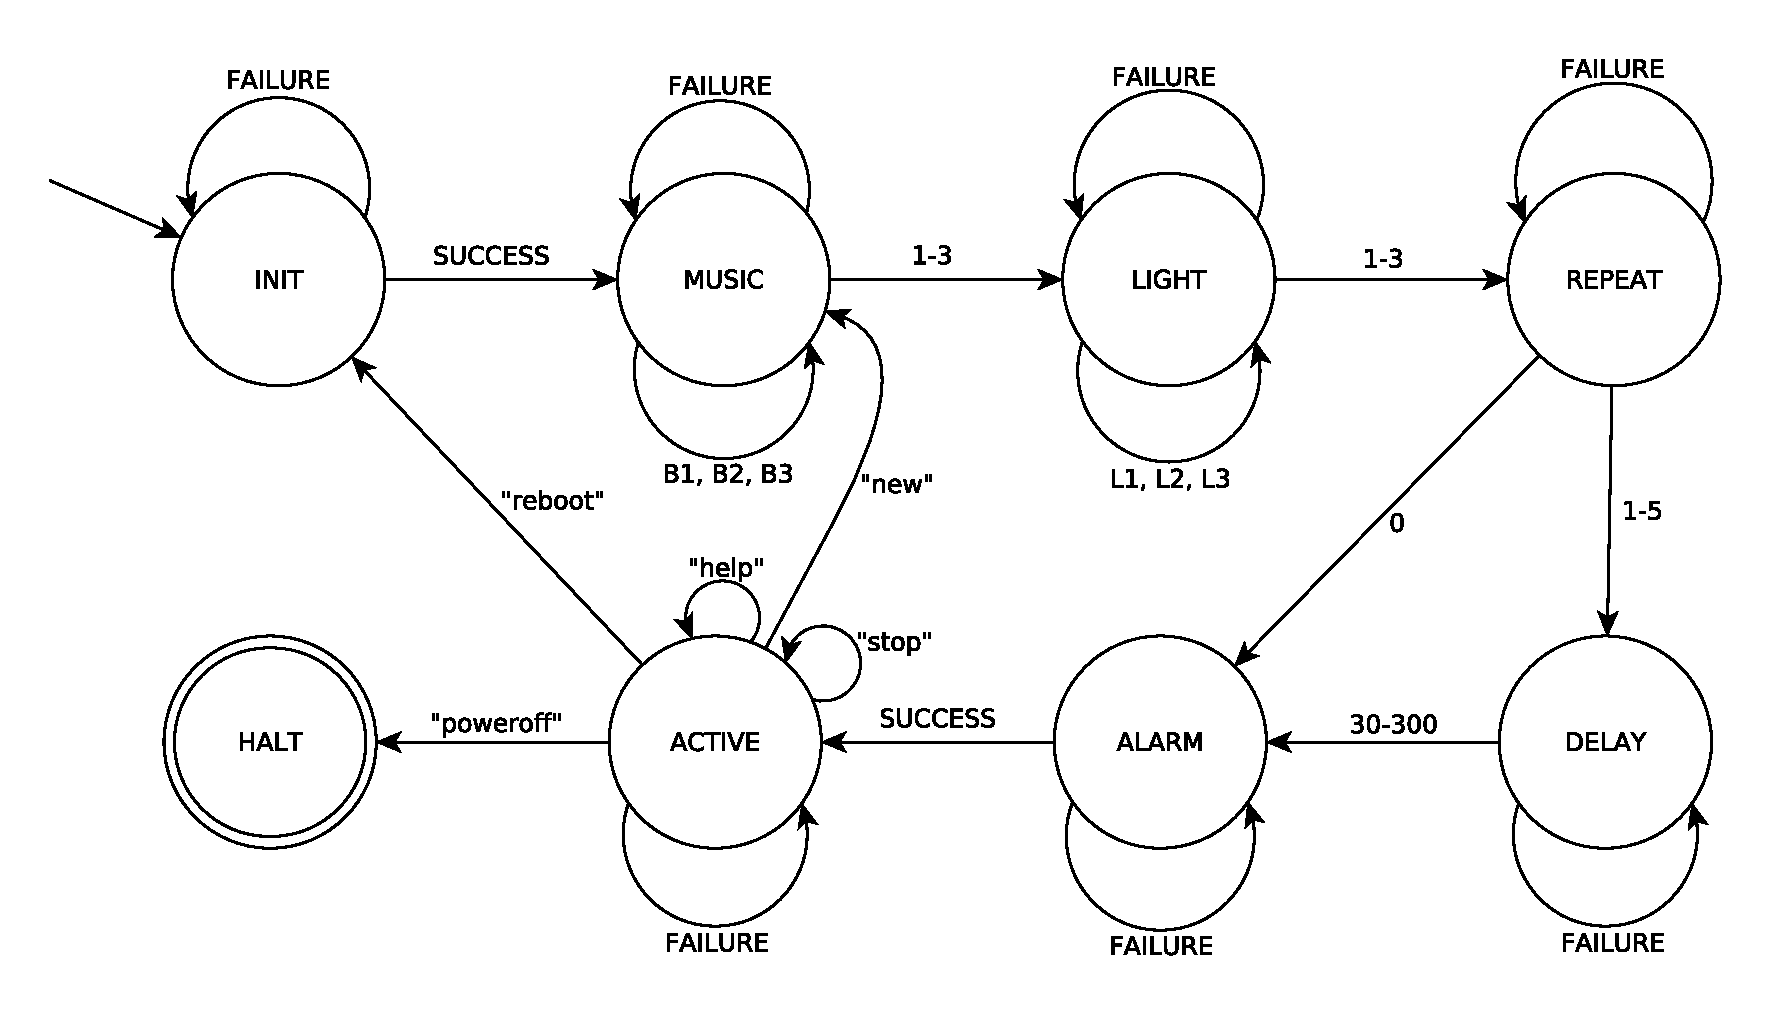
\includegraphics[scale=0.55]{img/fsm.eps}
    \caption{Budík - Konečný automat}
    \label{fig:fsm}
\end{figure}

\newpage %#########################################################################################

\makeatletter
\makeatother
\bibliographystyle{czechiso}
\begin{flushleft}
    \bibliography{quotation}
\end{flushleft}

\end{document} %###################################################################################


